\documentclass[12pt,a4paper]{article}
\usepackage{amsmath, amssymb, geometry, booktabs, xcolor, hyperref,
            listings, pgfplots, tcolorbox, enumitem, fancyhdr, tikz, array}
\usepgfplotslibrary{fillbetween}
\geometry{margin=2.5cm}
\pgfplotsset{compat=1.18}
\tcbuselibrary{skins, breakable}

% Define custom environments
\newtcolorbox{curiositybox}[1]{colback=yellow!10, colframe=orange!80, title=#1, breakable}
\newtcolorbox{infobox}[1]{colback=blue!5, colframe=blue!60, title=#1, breakable}
\newtcolorbox{mistakebox}[1]{colback=red!5, colframe=red!60, title=#1, breakable}
\newtcolorbox{learnbox}[1]{colback=green!5, colframe=green!60, title=#1, breakable}

% Header and Footer
\pagestyle{fancy}
\fancyhf{}
\lhead{Coordinate Systems}
\rhead{Unit 5 --- LAC}
\cfoot{\thepage}

% Document Title Setup
\title{\textbf{Coordinate Systems: Change of Variables, Polar, Cylindrical \& Spherical Coordinates} \\ \large Unit 5: Multiple Integrals and Coordinate Transformations}
\author{Department of Mathematics}
\date{\today}

\begin{document}
\maketitle
\tableofcontents
\newpage

%=============================================================
\section{Real-World Engineering Hook}
%=============================================================

\begin{curiositybox}{Why Should an Engineer Care?}
Imagine you are computing the gravitational field of a uniform solid sphere of radius $R$ and density $\delta$.
In Cartesian coordinates, the region is $x^2 + y^2 + z^2 \leq R^2$, and the limits become
\[
  -R \leq x \leq R, \quad -\sqrt{R^2 - x^2} \leq y \leq \sqrt{R^2 - x^2}, \quad
  -\sqrt{R^2 - x^2 - y^2} \leq z \leq \sqrt{R^2 - x^2 - y^2}.
\]
These nested square-root limits make the integral essentially impossible to evaluate by hand and extremely error-prone
in software. Switch to spherical coordinates $(\rho, \phi, \theta)$ and the same region becomes simply
$0 \leq \rho \leq R$, $0 \leq \phi \leq \pi$, $0 \leq \theta \leq 2\pi$ --- three constant-limit integrals that
factor cleanly.

Similarly, analyzing current density in a cylindrical copper conductor (skin effect in AC circuits) requires
integrating over a disk cross-section. Polar limits $0 \leq r \leq a$, $0 \leq \theta \leq 2\pi$ replace
unwieldy Cartesian square-root bounds. And computing the pressure distribution over a circular turbine blade
cross-section demands the polar Jacobian factor $r$ in $dA = r\,dr\,d\theta$ --- forget it, and your computed
force integral is wrong by an infinite factor as $r \to 0$.

The key insight is: \textbf{every coordinate change multiplies the integrand by the Jacobian determinant $|J|$},
which accounts for the distortion of area or volume elements. Choosing the right system is not a luxury --- it is
the difference between a 3-line calculation and an intractable mess.
\end{curiositybox}

%=============================================================
\section{Why This Topic Exists}
%=============================================================

\begin{center}
\begin{tabular}{>{\bfseries}p{5cm} p{9cm}}
\toprule
\textbf{Theoretical Concept} & \textbf{Engineering Application / Consequence of Misunderstanding} \\
\midrule
General Jacobian (change of variables) & Finite element mesh mapping --- wrong Jacobian yields physically
  incorrect stiffness matrix entries, causing structural simulations to predict false deflections. \\
\addlinespace
Polar coordinates & Pressure or flux over circular/annular cross-sections --- Cartesian limits produce
  nested radicals that are unmanageable for disks or washers. \\
\addlinespace
Cylindrical coordinates & Heat conduction in cylindrical pipes --- cylindrical coordinates decouple the
  radial and axial dependencies, dramatically simplifying the governing PDE solutions. \\
\addlinespace
Spherical coordinates & Gravitational and electrostatic potential around spherical bodies --- natural
  symmetry alignment reduces triple integrals to three independent single integrals. \\
\bottomrule
\end{tabular}
\end{center}

\vspace{0.5em}
\begin{learnbox}{Core Learning Objective}
By the end of this topic you will be able to:
\begin{itemize}[leftmargin=1.5em]
  \item State the general change-of-variables formula and compute the Jacobian determinant.
  \item Convert double and triple integrals to polar, cylindrical, and spherical coordinates.
  \item Identify which coordinate system matches a given region's geometry.
  \item Write the correct area/volume element including the Jacobian factor for each system.
\end{itemize}
\end{learnbox}

%=============================================================
\section{Intuition First \& Mathematical Definitions}
%=============================================================

\subsection{Change of Variables and the Jacobian Determinant}

Think of a coordinate transformation as a \emph{stretching and shearing} of the plane. When you map
a simple region $S$ in the $(u,v)$-plane to a complicated region $R$ in the $(x,y)$-plane via
$x = g(u,v)$, $y = h(u,v)$, small area patches get distorted. The Jacobian determinant $J$ measures
exactly how much a unit patch in $(u,v)$ has been magnified or shrunk when mapped to $(x,y)$. If
$|J| = 3$, a $1 \times 1$ square in $uv$-space becomes a region of area 3 in $xy$-space --- so you
\emph{must} multiply the integrand by $|J|$ to keep the integral correct.

\begin{infobox}{Change of Variables --- Jacobian Transformation}
Let $x = g(u,v)$, $y = h(u,v)$ be a one-to-one differentiable transformation mapping region $S$ in
the $(u,v)$-plane onto region $R$ in the $(x,y)$-plane. The \textbf{Jacobian determinant} is
\[
  J = \frac{\partial(x,y)}{\partial(u,v)}
    = \begin{vmatrix} \dfrac{\partial x}{\partial u} & \dfrac{\partial x}{\partial v} \\[8pt]
                      \dfrac{\partial y}{\partial u} & \dfrac{\partial y}{\partial v} \end{vmatrix}
    = \frac{\partial x}{\partial u}\frac{\partial y}{\partial v}
      - \frac{\partial x}{\partial v}\frac{\partial y}{\partial u}.
\]
\textbf{Change-of-Variables Formula:}
\[
  \iint_R f(x,y)\,dA = \iint_S f\bigl(g(u,v),\,h(u,v)\bigr)\,\bigl|J\bigr|\,du\,dv.
\]
\textbf{Key notes:}
\begin{itemize}[leftmargin=1.5em]
  \item $|J|$ is the absolute value of the Jacobian --- area elements are always positive.
  \item If $J = 0$ at a point, the transformation is not one-to-one there (degenerate); the formula
        breaks down and those points must be handled carefully (they form a set of measure zero in
        most practical cases).
  \item The inverse Jacobian satisfies $\partial(u,v)/\partial(x,y) = 1/J$ when $J \neq 0$.
  \item For triple integrals: $\iiint_R f\,dV = \iiint_S f\,|J_3|\,du\,dv\,dw$ where
        $J_3 = \partial(x,y,z)/\partial(u,v,w)$ is the $3\times3$ determinant.
\end{itemize}
\end{infobox}

\textbf{Worked Example 3.1 (General Jacobian --- Ellipse):}
Evaluate $\iint_R dA$ where $R$ is the region $\dfrac{x^2}{9} + \dfrac{y^2}{4} \leq 1$.

\textit{Solution.} Use the substitution $x = 3u$, $y = 2v$. Then
\[
  \frac{\partial x}{\partial u} = 3,\quad \frac{\partial x}{\partial v} = 0,\quad
  \frac{\partial y}{\partial u} = 0,\quad \frac{\partial y}{\partial v} = 2.
\]
\[
  J = \begin{vmatrix} 3 & 0 \\ 0 & 2 \end{vmatrix} = 3 \cdot 2 - 0 \cdot 0 = 6.
\]
The ellipse $\tfrac{x^2}{9}+\tfrac{y^2}{4}\leq1$ becomes the unit disk $u^2 + v^2 \leq 1$ in $(u,v)$.
\[
  \iint_R dA = \iint_{u^2+v^2\leq1} 1 \cdot |J|\,du\,dv = 6 \iint_{u^2+v^2\leq1} du\,dv
             = 6 \cdot \pi(1)^2 = 6\pi.
\]
(The area of an ellipse with semi-axes $a=3$, $b=2$ is $\pi ab = 6\pi$. \checkmark)

%-------------------------------------------------------------
\subsection{Polar Coordinates}

When a region is a disk, annulus, or sector --- anything described more naturally by distance from
the origin and angle than by horizontal and vertical extents --- polar coordinates are the right
choice. The $r$ factor that appears in $dA = r\,dr\,d\theta$ is not optional; it is precisely the
Jacobian of the polar transformation and reflects the geometric fact that a thin ring of radius $r$
and angular width $d\theta$ has arc length $r\,d\theta$, so its area is $r\,dr\,d\theta$.

\begin{infobox}{Polar Coordinates}
\textbf{Transformation:}
\[
  x = r\cos\theta, \qquad y = r\sin\theta, \qquad r \geq 0,\; 0 \leq \theta \leq 2\pi.
\]
\textbf{Jacobian:}
\[
  J = \frac{\partial(x,y)}{\partial(r,\theta)}
    = \begin{vmatrix} \cos\theta & -r\sin\theta \\ \sin\theta & r\cos\theta \end{vmatrix}
    = r\cos^2\theta + r\sin^2\theta = r.
\]
Therefore $|J| = r$ and the \textbf{area element} is
\[
  dA = r\,dr\,d\theta.
\]
\textbf{Double integral in polar form:}
\[
  \iint_R f(x,y)\,dA = \int_{\alpha}^{\beta}\int_{r_1(\theta)}^{r_2(\theta)}
      f(r\cos\theta,\, r\sin\theta)\; r\,dr\,d\theta.
\]
\textbf{Key identities:} $r^2 = x^2 + y^2$; $\theta = \arctan(y/x)$; $x^2+y^2 = r^2$.
\end{infobox}

\textbf{Worked Example 3.2 (Polar --- Unit Disk):}
Evaluate $\displaystyle\iint_R \sqrt{x^2+y^2}\,dA$ where $R$ is the disk $x^2+y^2 \leq 9$.

\textit{Solution.}  In polar coordinates $\sqrt{x^2+y^2} = r$ and the disk is $0 \leq r \leq 3$,
$0 \leq \theta \leq 2\pi$.
\[
  \iint_R \sqrt{x^2+y^2}\,dA
  = \int_0^{2\pi}\int_0^3 r \cdot r\,dr\,d\theta
  = \int_0^{2\pi}\int_0^3 r^2\,dr\,d\theta.
\]
Inner integral: $\displaystyle\int_0^3 r^2\,dr = \left[\frac{r^3}{3}\right]_0^3 = \frac{27}{3} = 9$.

Outer integral: $\displaystyle\int_0^{2\pi} 9\,d\theta = 9 \cdot 2\pi = 18\pi$.

\[
  \boxed{\iint_R \sqrt{x^2+y^2}\,dA = 18\pi.}
\]

%-------------------------------------------------------------
\subsection{Cylindrical Coordinates}

Cylindrical coordinates extend polar coordinates to three dimensions by simply appending the vertical
coordinate $z$. The cross-section in the $xy$-plane uses $(r,\theta)$ exactly as before, while $z$
runs independently along the vertical axis. This makes cylindrical coordinates ideal for any solid
that has a circular cross-section at each height level --- pipes, cylinders, cones, paraboloids.

\begin{infobox}{Cylindrical Coordinates}
\textbf{Transformation:}
\[
  x = r\cos\theta, \qquad y = r\sin\theta, \qquad z = z,
\]
where $r \geq 0$, $0 \leq \theta \leq 2\pi$, $-\infty < z < \infty$.

\textbf{Jacobian:}
\[
  J_3 = \frac{\partial(x,y,z)}{\partial(r,\theta,z)}
      = \begin{vmatrix}
          \cos\theta & -r\sin\theta & 0 \\
          \sin\theta & r\cos\theta  & 0 \\
          0          & 0            & 1
        \end{vmatrix}
      = 1 \cdot (r\cos^2\theta + r\sin^2\theta) = r.
\]
\textbf{Volume element:}
\[
  dV = r\,dr\,d\theta\,dz.
\]
\textbf{Triple integral in cylindrical form:}
\[
  \iiint_E f(x,y,z)\,dV
  = \int_{\alpha}^{\beta}\int_{r_1}^{r_2}\int_{z_1(r,\theta)}^{z_2(r,\theta)}
      f(r\cos\theta,\,r\sin\theta,\,z)\;r\,dz\,dr\,d\theta.
\]
\textbf{Note:} The cylinder $x^2+y^2 = a^2$ becomes simply $r = a$ in cylindrical coordinates.
\end{infobox}

\textbf{Worked Example 3.3 (Cylindrical --- Volume of a Paraboloid Cap):}
Find the volume of the solid bounded above by $z = 4 - r^2$ (i.e.\ $z = 4 - x^2 - y^2$),
below by $z = 0$, and inside $r \leq 2$.

\textit{Solution.}  The solid is $0 \leq \theta \leq 2\pi$, $0 \leq r \leq 2$, $0 \leq z \leq 4-r^2$.
\[
  V = \int_0^{2\pi}\int_0^2\int_0^{4-r^2} r\,dz\,dr\,d\theta.
\]
Innermost (over $z$):
\[
  \int_0^{4-r^2} dz = 4 - r^2.
\]
Middle (over $r$):
\[
  \int_0^2 r(4 - r^2)\,dr = \int_0^2 (4r - r^3)\,dr
  = \left[2r^2 - \frac{r^4}{4}\right]_0^2 = 2(4) - \frac{16}{4} = 8 - 4 = 4.
\]
Outermost (over $\theta$):
\[
  \int_0^{2\pi} 4\,d\theta = 8\pi.
\]
\[
  \boxed{V = 8\pi.}
\]

%-------------------------------------------------------------
\subsection{Spherical Coordinates}

When a solid is bounded by a sphere or exhibits a three-dimensional radial symmetry, spherical
coordinates eliminate every square root that would appear in Cartesian limits. The variable $\rho$
measures distance from the origin, $\phi$ is the polar angle measured from the positive $z$-axis
(colatitude), and $\theta$ is the azimuthal angle in the $xy$-plane, identical to polar. The
Jacobian $\rho^2\sin\phi$ grows with $\rho^2$ because spherical ``shells'' at larger radius enclose
more volume per unit $\rho$-increment.

\begin{infobox}{Spherical Coordinates}
\textbf{Transformation:}
\[
  x = \rho\sin\phi\cos\theta, \qquad y = \rho\sin\phi\sin\theta, \qquad z = \rho\cos\phi,
\]
where $\rho \geq 0$, $0 \leq \phi \leq \pi$, $0 \leq \theta \leq 2\pi$.

\textbf{Jacobian:}
\[
  J_3 = \frac{\partial(x,y,z)}{\partial(\rho,\phi,\theta)} = \rho^2\sin\phi.
\]
\textbf{Volume element:}
\[
  dV = \rho^2\sin\phi\,d\rho\,d\phi\,d\theta.
\]
\textbf{Triple integral in spherical form:}
\[
  \iiint_E f(x,y,z)\,dV
  = \int_0^{2\pi}\int_0^{\pi}\int_0^{R}
      f(\rho\sin\phi\cos\theta,\,\rho\sin\phi\sin\theta,\,\rho\cos\phi)\;
      \rho^2\sin\phi\,d\rho\,d\phi\,d\theta.
\]
\textbf{Key identity:} $x^2 + y^2 + z^2 = \rho^2$.\\
\textbf{Ranges:} $\rho \in [0,\infty)$; $\phi \in [0,\pi]$ (not $2\pi$); $\theta \in [0,2\pi)$.
\end{infobox}

\textbf{Worked Example 3.4 (Spherical --- Volume of a Sphere):}
Find the volume of the ball $x^2+y^2+z^2 \leq a^2$ using spherical coordinates.

\textit{Solution.}  The ball is $0 \leq \rho \leq a$, $0 \leq \phi \leq \pi$, $0 \leq \theta \leq 2\pi$.
\[
  V = \int_0^{2\pi}\int_0^{\pi}\int_0^a \rho^2\sin\phi\,d\rho\,d\phi\,d\theta.
\]
Innermost (over $\rho$):
\[
  \int_0^a \rho^2\,d\rho = \frac{a^3}{3}.
\]
Middle (over $\phi$):
\[
  \int_0^{\pi} \sin\phi\,d\phi = \bigl[-\cos\phi\bigr]_0^{\pi} = -\cos\pi + \cos 0 = 1 + 1 = 2.
\]
Outermost (over $\theta$):
\[
  \int_0^{2\pi} d\theta = 2\pi.
\]
\[
  V = \frac{a^3}{3} \cdot 2 \cdot 2\pi = \frac{4\pi a^3}{3}. \qquad \checkmark
\]
\[
  \boxed{V = \tfrac{4}{3}\pi a^3.}
\]

%=============================================================
\section{Visual Artifacts \& Geometric Interpretation}
%=============================================================

\subsection*{Diagram 1: Polar Coordinate Grid vs.\ Cartesian Grid}

\begin{center}
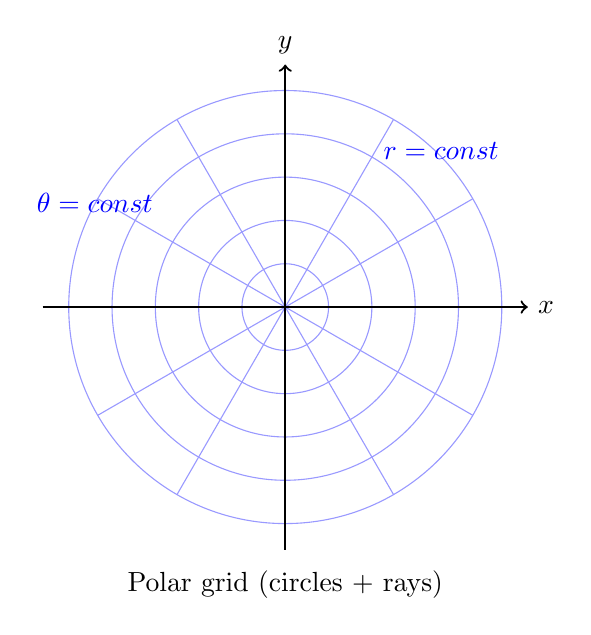
\begin{tikzpicture}[scale=1.1]
  % Polar grid
  \foreach \r in {0.5,1,1.5,2,2.5}{
    \draw[blue!40, thin] (0,0) circle (\r);
  }
  \foreach \ang in {0,30,...,330}{
    \draw[blue!40, thin] (0,0) -- ({2.5*cos(\ang)},{2.5*sin(\ang)});
  }
  \draw[->, thick] (-2.8,0) -- (2.8,0) node[right] {$x$};
  \draw[->, thick] (0,-2.8) -- (0,2.8) node[above] {$y$};
  \node[blue] at (1.8,1.8) {$r=const$};
  \node[blue] at (-2.2,1.2) {$\theta=const$};
  \node at (0,-3.2) {Polar grid (circles + rays)};
\end{tikzpicture}
\hspace{1.5cm}
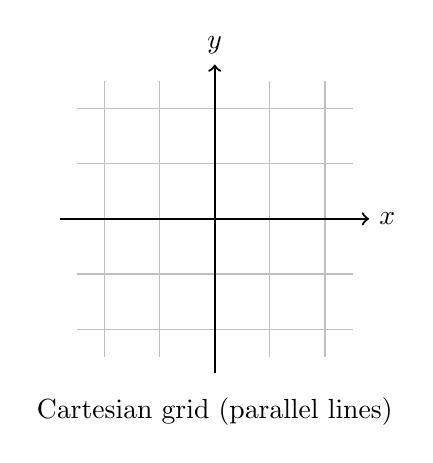
\begin{tikzpicture}[scale=0.7]
  % Cartesian grid
  \foreach \x in {-2,-1,0,1,2}{
    \draw[gray!50] (\x,-2.5) -- (\x,2.5);
  }
  \foreach \y in {-2,-1,0,1,2}{
    \draw[gray!50] (-2.5,\y) -- (2.5,\y);
  }
  \draw[->, thick] (-2.8,0) -- (2.8,0) node[right] {$x$};
  \draw[->, thick] (0,-2.8) -- (0,2.8) node[above] {$y$};
  \node at (0,-3.5) {Cartesian grid (parallel lines)};
\end{tikzpicture}
\end{center}

\subsection*{Diagram 2: Cylindrical Coordinate Volume Element}

\begin{center}
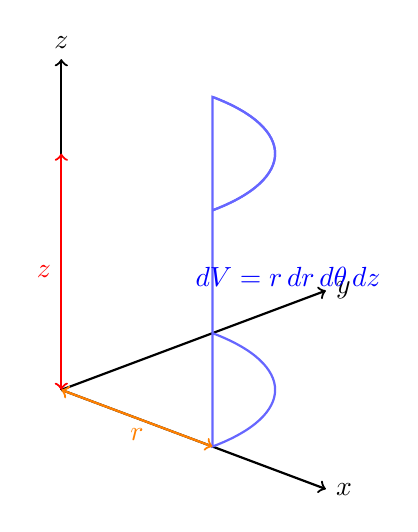
\begin{tikzpicture}[x={(0.8cm,-0.3cm)}, y={(0.8cm,0.3cm)}, z={(0cm,1cm)}, scale=1.2]
  % Axes
  \draw[->, thick] (0,0,0) -- (3.5,0,0) node[right] {$x$};
  \draw[->, thick] (0,0,0) -- (0,3.5,0) node[right] {$y$};
  \draw[->, thick] (0,0,0) -- (0,0,3.5) node[above] {$z$};
  % Cylinder outline
  \draw[blue!60, thick] (2,0,0) arc (0:90:2) -- (0,2,2.5) arc (90:0:2) -- cycle;
  \draw[blue!60, thick] (2,0,2.5) arc (0:90:2);
  % Labels
  \draw[<->, orange, thick] (0,0,0) -- (2,0,0) node[midway, below] {$r$};
  \draw[<->, red, thick] (0,0,0) -- (0,0,2.5) node[midway, left] {$z$};
  \node[blue] at (1.5,1.5,1.2) {$dV=r\,dr\,d\theta\,dz$};
\end{tikzpicture}
\end{center}

\subsection*{Diagram 3: Spherical Coordinate Volume Element}

\begin{center}
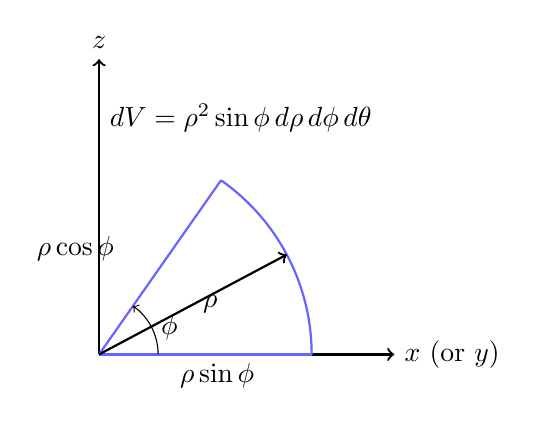
\begin{tikzpicture}[scale=1.5]
  % Axes
  \draw[->, thick] (0,0) -- (2.5,0) node[right] {$x$ (or $y$)};
  \draw[->, thick] (0,0) -- (0,2.5) node[above] {$z$};
  % Sphere arc
  \draw[blue!60, thick] (0,0) -- (1.8,0);
  \draw[blue!60, thick] (0,0) -- ({1.8*cos(55)},{1.8*sin(55)});
  \draw[blue!60, thick] (1.8,0) arc (0:55:1.8);
  % Labels
  \node at (1.0,-0.18) {$\rho\sin\phi$};
  \node at (-0.2,0.9) {$\rho\cos\phi$};
  \draw[->, thick] (0,0) -- ({1.8*cos(28)},{1.8*sin(28)}) node[midway, right] {$\rho$};
  \draw[->] (0.5,0) arc (0:55:0.5) node[midway, right] {$\phi$};
  \node at (1.2,2.0) {$dV = \rho^2\sin\phi\,d\rho\,d\phi\,d\theta$};
\end{tikzpicture}
\end{center}

\subsection*{Diagram 4: Jacobian $|J|=r$ grows linearly with $r$}

\begin{center}
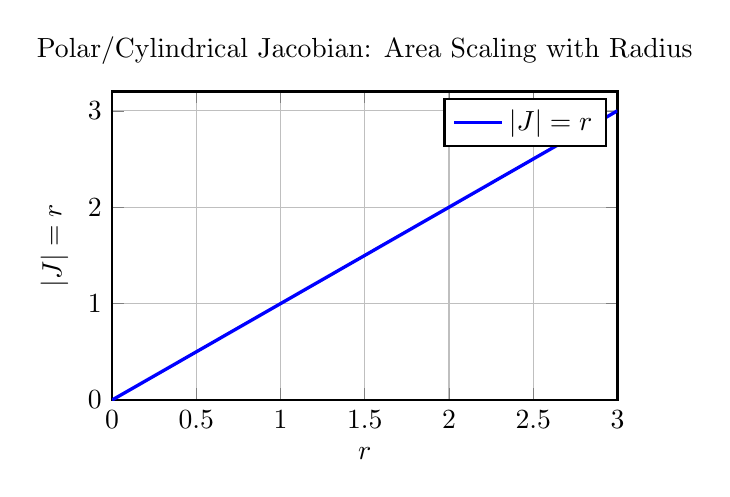
\begin{tikzpicture}
\begin{axis}[
  xlabel={$r$},
  ylabel={$|J| = r$},
  title={Polar/Cylindrical Jacobian: Area Scaling with Radius},
  xmin=0, xmax=3, ymin=0, ymax=3.2,
  width=8cm, height=5.5cm,
  grid=major,
  thick
]
  \addplot[blue, very thick, domain=0:3, samples=60] {x};
  \addlegendentry{$|J|=r$}
\end{axis}
\end{tikzpicture}
\end{center}
A ring at radius $r=2$ has twice the arc length (and twice the area element) as a ring at $r=1$ for
the same $dr$ and $d\theta$ increments, which is exactly what $|J|=r$ encodes.

%=============================================================
\section{Step-by-Step Algorithmic Workflow}
%=============================================================

\begin{infobox}{Algorithm: Evaluating an Integral in a New Coordinate System}
\textbf{Step 1 --- Identify symmetry.}
Inspect the region $R$ and integrand $f$:
\begin{itemize}[leftmargin=1.5em]
  \item Disk/annulus or $x^2+y^2$ in 2D $\Rightarrow$ \textbf{Polar}.
  \item Cylinder, cone, paraboloid of revolution $\Rightarrow$ \textbf{Cylindrical}.
  \item Sphere, hemisphere, spherical shell $\Rightarrow$ \textbf{Spherical}.
  \item Parallelogram, ellipse, linear region $\Rightarrow$ \textbf{General change of variables}.
\end{itemize}

\textbf{Step 2 --- Write the transformation equations.}
State $x=g(u,v)$, $y=h(u,v)$ (and $z$ if needed). Verify the transformation is one-to-one on the
interior of $S$.

\textbf{Step 3 --- Compute the Jacobian determinant.}
Form the matrix of partial derivatives and compute its determinant. Simplify; take absolute value.

\textbf{Step 4 --- Express the integrand.}
Substitute $x = g(u,v)$, $y = h(u,v)$ (and $z$) into $f(x,y,z)$ and simplify.

\textbf{Step 5 --- Set up new limits.}
Find what the boundary of $R$ in $(x,y)$ becomes in $(u,v)$. Determine the new limits by examining
the transformed region $S$ systematically (sketch if needed).

\textbf{Step 6 --- Evaluate the transformed integral.}
Multiply integrand by $|J|$, write the iterated integral with new limits, and integrate from inside
out.

\textbf{Decision Table:}
\begin{center}
\begin{tabular}{lll}
\toprule
\textbf{Region shape} & \textbf{Key feature} & \textbf{Use} \\
\midrule
Disk / annulus (2D) & $x^2+y^2 = c$ boundary & Polar \\
Cylinder / cone (3D) & Circular cross-section & Cylindrical \\
Sphere / hemisphere (3D) & $x^2+y^2+z^2 = c$ boundary & Spherical \\
Ellipse / parallelogram & Linear or quadratic boundary & General Jacobian \\
Rectangle in $(u,v)$ & After linear substitution & General Jacobian \\
\bottomrule
\end{tabular}
\end{center}
\end{infobox}

%=============================================================
\section{Fully Worked Step-by-Step Numerical Examples}
%=============================================================

\subsection*{Example 1 --- Polar (Gaussian Integral over the Unit Disk)}

Evaluate $\displaystyle I = \iint_R e^{-(x^2+y^2)}\,dA$ where $R$ is the unit disk $x^2+y^2 \leq 1$.

\textit{Step 1.}  The region $R$ is a disk. Use polar coordinates: $x = r\cos\theta$, $y = r\sin\theta$,
$dA = r\,dr\,d\theta$.

\textit{Step 2.}  Region: $0 \leq r \leq 1$, $0 \leq \theta \leq 2\pi$.

\textit{Step 3.}  Integrand: $x^2+y^2 = r^2$, so $e^{-(x^2+y^2)} = e^{-r^2}$.

\textit{Step 4.}  Set up:
\[
  I = \int_0^{2\pi}\int_0^1 e^{-r^2} \cdot r\,dr\,d\theta.
\]
\textit{Step 5.}  Inner integral over $r$ (substitute $t = r^2$, $dt = 2r\,dr$):
\[
  \int_0^1 r e^{-r^2}\,dr = \frac{1}{2}\int_0^1 e^{-t}\,dt
  = \frac{1}{2}\bigl[-e^{-t}\bigr]_0^1
  = \frac{1}{2}(1 - e^{-1})
  = \frac{1}{2}\!\left(1 - \frac{1}{e}\right).
\]
\textit{Step 6.}  Outer integral over $\theta$:
\[
  I = \int_0^{2\pi} \frac{1}{2}\!\left(1 - \frac{1}{e}\right)d\theta
    = \frac{1}{2}\!\left(1 - \frac{1}{e}\right) \cdot 2\pi
    = \pi\!\left(1 - \frac{1}{e}\right).
\]
\[
  \boxed{I = \pi\!\left(1 - e^{-1}\right) \approx 1.986.}
\]

\begin{learnbox}{Insight for Example 1}
Notice that $e^{-(x^2+y^2)} = e^{-r^2}$ in polar form --- a function that depends only on radius
is always separable in polar coordinates, making the integral straightforward.
\end{learnbox}

\subsection*{Example 2 --- Cylindrical (Volume inside Cylinder below Cone)}

Find the volume of the solid inside the cylinder $x^2+y^2 = 4$ (i.e.\ $r=2$), above $z=0$, and
below $z = 3 - r$ (where $r = \sqrt{x^2+y^2}$).

\textit{Step 1.}  The region has circular symmetry. Use cylindrical coordinates.

\textit{Step 2.}  Range: $0 \leq \theta \leq 2\pi$, $0 \leq r \leq 2$, $0 \leq z \leq 3-r$.
We need $3-r \geq 0$, i.e.\ $r \leq 3$; since $r \leq 2$ this is automatically satisfied.

\textit{Step 3.}
\[
  V = \int_0^{2\pi}\int_0^2\int_0^{3-r} r\,dz\,dr\,d\theta.
\]
\textit{Step 4.}  Innermost over $z$:
\[
  \int_0^{3-r} dz = 3 - r.
\]
\textit{Step 5.}  Middle over $r$:
\[
  \int_0^2 r(3-r)\,dr = \int_0^2(3r - r^2)\,dr
  = \left[\frac{3r^2}{2} - \frac{r^3}{3}\right]_0^2
  = \frac{3 \cdot 4}{2} - \frac{8}{3}
  = 6 - \frac{8}{3}
  = \frac{18-8}{3} = \frac{10}{3}.
\]
\textit{Step 6.}  Outer over $\theta$:
\[
  V = \int_0^{2\pi}\frac{10}{3}\,d\theta = \frac{10}{3} \cdot 2\pi = \frac{20\pi}{3}.
\]
\[
  \boxed{V = \frac{20\pi}{3} \approx 20.94 \text{ cubic units.}}
\]

\begin{learnbox}{Insight for Example 2}
The upper surface $z = 3-r$ is a cone in disguise. In cylindrical coordinates its equation is linear
in $r$ and $z$, making limit setup straightforward --- in Cartesian it would involve $\sqrt{x^2+y^2}$.
\end{learnbox}

\subsection*{Example 3 --- Spherical (Mass of a Hemisphere with Variable Density)}

Compute the mass of a solid hemisphere $x^2+y^2+z^2 \leq a^2$, $z \geq 0$, with density
$\delta(x,y,z) = k z$ (density proportional to height; models sedimentation in a hemispherical tank).

\textit{Step 1.}  The region is a hemisphere. Use spherical coordinates. In spherical form,
$z = \rho\cos\phi$ and the hemisphere is $0 \leq \rho \leq a$, $0 \leq \phi \leq \pi/2$,
$0 \leq \theta \leq 2\pi$.

\textit{Step 2.}  Density: $\delta = kz = k\rho\cos\phi$.

\textit{Step 3.}
\[
  M = \iiint_E kz\,dV
    = \int_0^{2\pi}\int_0^{\pi/2}\int_0^a
        k\rho\cos\phi \cdot \rho^2\sin\phi\,d\rho\,d\phi\,d\theta.
\]
\textit{Step 4.}  Innermost over $\rho$:
\[
  \int_0^a k\rho^3\cos\phi\sin\phi\,d\rho
  = k\cos\phi\sin\phi \cdot \frac{a^4}{4}.
\]
\textit{Step 5.}  Middle over $\phi$:
\[
  \int_0^{\pi/2}\frac{k a^4}{4}\cos\phi\sin\phi\,d\phi
  = \frac{k a^4}{4}\int_0^{\pi/2}\frac{\sin 2\phi}{2}\,d\phi
  = \frac{k a^4}{8}\left[-\frac{\cos 2\phi}{2}\right]_0^{\pi/2}
  = \frac{k a^4}{8}\cdot\frac{-\cos\pi + \cos 0}{2}
  = \frac{k a^4}{8}\cdot\frac{1+1}{2}
  = \frac{k a^4}{8}.
\]
\textit{Step 6.}  Outer over $\theta$:
\[
  M = \int_0^{2\pi}\frac{k a^4}{8}\,d\theta = \frac{k a^4}{8}\cdot 2\pi = \frac{\pi k a^4}{4}.
\]
\[
  \boxed{M = \frac{\pi k a^4}{4}.}
\]
\textit{Interpretation:} The mass scales as $a^4$ (not $a^3$) because the density $kz$ itself grows
with the size of the hemisphere. For $a = 1$, $k = 1$: $M = \pi/4 \approx 0.785$ mass units.

\begin{learnbox}{Insight for Example 3}
The factor $\rho^2\sin\phi$ in the spherical volume element is \emph{not} optional --- it converts
the $d\rho\,d\phi\,d\theta$ box into actual physical volume. Without it, the computed mass would be
dimensionally and numerically wrong.
\end{learnbox}

\subsection*{Example 4 --- General Change of Variables (Elliptical Region)}

Evaluate $\displaystyle I = \iint_R (x + y)\,dA$ where $R$ is the ellipse $\dfrac{x^2}{4} + y^2 \leq 1$.

\textit{Step 1.}  Use the substitution $x = 2u$, $y = v$. Then the ellipse becomes the unit disk
$u^2 + v^2 \leq 1$ in the $(u,v)$-plane.

\textit{Step 2.}  Compute the Jacobian:
\[
  \frac{\partial x}{\partial u} = 2,\quad \frac{\partial x}{\partial v} = 0,\quad
  \frac{\partial y}{\partial u} = 0,\quad \frac{\partial y}{\partial v} = 1.
\]
\[
  J = \begin{vmatrix} 2 & 0 \\ 0 & 1 \end{vmatrix} = 2 - 0 = 2, \qquad |J| = 2.
\]
\textit{Step 3.}  Integrand: $x + y = 2u + v$.

\textit{Step 4.}
\[
  I = \iint_{u^2+v^2 \leq 1} (2u + v) \cdot 2\,du\,dv
    = 2\iint_{u^2+v^2\leq1} (2u + v)\,du\,dv.
\]
\textit{Step 5.}  Now switch the unit disk to polar: $u = r\cos\alpha$, $v = r\sin\alpha$,
$du\,dv = r\,dr\,d\alpha$, $0 \leq r \leq 1$, $0 \leq \alpha \leq 2\pi$.
\[
  \iint_{u^2+v^2\leq1}2u\,du\,dv
  = \int_0^{2\pi}\int_0^1 2r\cos\alpha \cdot r\,dr\,d\alpha
  = 2\int_0^1 r^2\,dr \int_0^{2\pi}\cos\alpha\,d\alpha
  = 2 \cdot \frac{1}{3} \cdot 0 = 0.
\]
\[
  \iint_{u^2+v^2\leq1}v\,du\,dv
  = \int_0^{2\pi}\int_0^1 r\sin\alpha \cdot r\,dr\,d\alpha
  = \int_0^1 r^2\,dr \int_0^{2\pi}\sin\alpha\,d\alpha
  = \frac{1}{3}\cdot 0 = 0.
\]
(Both integrals vanish because $\int_0^{2\pi}\cos\alpha\,d\alpha = 0$ and
$\int_0^{2\pi}\sin\alpha\,d\alpha = 0$.)

\textit{Step 6.}
\[
  I = 2(0 + 0) = 0.
\]
\[
  \boxed{I = 0.}
\]
\textit{Geometric reason:} The integrand $x+y$ is an odd function over the ellipse (which is symmetric
about both axes), so the integral vanishes. The Jacobian $|J|=2$ is correct; it is the symmetry of
the domain that makes the result zero.

\begin{learnbox}{Insight for Example 4}
Even when the final answer is zero, the change-of-variables procedure must be carried out correctly:
compute $J$, transform the region, transform the integrand, and multiply by $|J|$. The method is
valid regardless of the numerical outcome.
\end{learnbox}

%=============================================================
\section{Tabular Reference: Coordinate System Comparison}
%=============================================================

\begin{center}
\begin{tabular}{p{2.8cm} p{3.5cm} p{2cm} p{2.5cm} p{3.5cm}}
\toprule
\textbf{System} & \textbf{Transformation} & \textbf{Jacobian} & \textbf{Element} & \textbf{Best Use / Engineering Example} \\
\midrule
\textbf{Polar (2D)} &
  $x = r\cos\theta$\newline $y = r\sin\theta$ &
  $|J| = r$ &
  $dA = r\,dr\,d\theta$ &
  Disk/annular regions; heat flux through circular cross-section \\
\addlinespace
\textbf{Cylindrical (3D)} &
  $x = r\cos\theta$\newline $y = r\sin\theta$\newline $z = z$ &
  $|J| = r$ &
  $dV = r\,dr\,d\theta\,dz$ &
  Cylindrical pipes, conical solids; current in a coaxial cable \\
\addlinespace
\textbf{Spherical (3D)} &
  $x = \rho\sin\phi\cos\theta$\newline $y = \rho\sin\phi\sin\theta$\newline $z = \rho\cos\phi$ &
  $|J| = \rho^2\sin\phi$ &
  $dV = \rho^2\sin\phi\,d\rho\,d\phi\,d\theta$ &
  Spherical bodies; gravitational potential of a planet \\
\addlinespace
\textbf{General (2D)} &
  $x = g(u,v)$\newline $y = h(u,v)$ &
  $\left|\dfrac{\partial(x,y)}{\partial(u,v)}\right|$ &
  $dA = |J|\,du\,dv$ &
  Elliptical regions, FEM mesh mappings, oblique transformations \\
\bottomrule
\end{tabular}
\end{center}

%=============================================================
\section{Common Student Mistakes \& Pitfalls}
%=============================================================

\begin{mistakebox}{Common Mistakes in Coordinate Transformations}
\begin{tabular}{>{\bfseries}p{4.5cm} p{4.5cm} p{5cm}}
\toprule
\textbf{Mistake} & \textbf{Why It Is Wrong} & \textbf{Correct Approach} \\
\midrule
Omitting the $r$ in $dA = dr\,d\theta$ (polar/cylindrical) &
  Forgets the Jacobian factor $|J|=r$; the area element in polar is not $dr\,d\theta$ &
  Always write $dA = r\,dr\,d\theta$ and $dV = r\,dr\,d\theta\,dz$; the extra $r$ is mandatory \\
\addlinespace
Writing $dV = \rho^2\sin\theta\,d\rho\,d\theta\,d\phi$ (mixing up $\phi$ and $\theta$) &
  $\phi$ is the polar angle from $z$-axis; $\theta$ is the azimuthal angle; $\sin\phi$ (not $\sin\theta$) appears in the Jacobian &
  Use $dV = \rho^2\sin\phi\,d\rho\,d\phi\,d\theta$; remember $\phi \in [0,\pi]$, $\theta \in [0,2\pi)$ \\
\addlinespace
Computing $J = \partial(u,v)/\partial(x,y)$ when $J = \partial(x,y)/\partial(u,v)$ is needed &
  These are reciprocals; using the inverse Jacobian gives an extra factor of $1/J^2$ error in the integral &
  Compute $J = \partial(x,y)/\partial(u,v)$ by differentiating the \emph{new} variables ($x,y$) with respect to the \emph{old} ($u,v$) \\
\addlinespace
Setting $\theta \in [0, \pi]$ instead of $[0, 2\pi]$ for a full disk/cylinder &
  Covers only the upper half of the disk, giving half the correct answer &
  A full circle requires $\theta \in [0, 2\pi]$; use $[0,\pi]$ only for a semicircle \\
\addlinespace
Setting $\phi \in [0, 2\pi]$ in spherical coordinates &
  $\phi$ is the colatitude and only ranges over $[0,\pi]$; values beyond $\pi$ repeat the same geometry &
  Keep $\phi \in [0,\pi]$ and $\theta \in [0,2\pi]$; do not confuse the roles of $\phi$ and $\theta$ \\
\bottomrule
\end{tabular}
\end{mistakebox}

%=============================================================
\section{Comprehensive Assessment Suite}
%=============================================================

\subsection*{Viva-Voce Questions}

\begin{enumerate}[label=\textbf{V\arabic*.}, leftmargin=2em]

\item \textbf{(Change of Variables)} What is the geometric meaning of the Jacobian determinant
  $|J| = |\partial(x,y)/\partial(u,v)|$? If $|J|=5$ at a point, what does this imply about areas
  of small patches near that point?

\item \textbf{(Change of Variables)} When does $J = 0$, and what goes wrong with the
  change-of-variables formula at such points? Give a concrete example.

\item \textbf{(Polar)} Explain in geometrical terms why the factor $r$ must appear in
  $dA = r\,dr\,d\theta$. Sketch the area of a thin polar strip and identify each factor.

\item \textbf{(Polar)} What are the standard polar limits for the upper half of the annulus
  $1 \leq x^2+y^2 \leq 4$, $y \geq 0$? Write them explicitly.

\item \textbf{(Cylindrical)} How does cylindrical coordinate differ from polar coordinates?
  Which additional variable is introduced, and what is its range for a cylinder of height $H$?

\item \textbf{(Spherical)} State the ranges of $\rho$, $\phi$, and $\theta$ for a full sphere
  of radius $R$. Why is $\phi$ limited to $[0,\pi]$ rather than $[0, 2\pi]$?

\item \textbf{(Spherical)} The volume element in spherical coordinates is
  $dV = \rho^2\sin\phi\,d\rho\,d\phi\,d\theta$. Explain why the factor $\sin\phi$ is present.
  What happens to this factor at $\phi = 0$ (north pole) and $\phi = \pi$ (south pole)?

\item \textbf{(General)} An engineer needs to integrate over the interior of the ellipse
  $x^2/a^2 + y^2/b^2 \leq 1$. Suggest an appropriate substitution and compute its Jacobian.

\end{enumerate}

\subsection*{Descriptive Exam Questions}

\begin{enumerate}[label=\textbf{D\arabic*.}, leftmargin=2em]

\item \textbf{[Polar, 8 marks]} Evaluate $\displaystyle\iint_R e^{-(x^2+y^2)}\,dA$ over the disk
  $x^2+y^2 \leq 4$ using polar coordinates. Show the limit setup, the Jacobian, and all integration
  steps. \\
  \textit{Hint:} Let $t = r^2$; evaluate the inner integral first.

\item \textbf{[Cylindrical, 10 marks]} Find the volume of the solid bounded by the paraboloid
  $z = x^2+y^2$ (below) and the plane $z = 4$ (above). Set up and evaluate the triple integral in
  cylindrical coordinates. \\
  \textit{Hint:} The two surfaces intersect where $r^2 = 4$, i.e.\ $r = 2$.

\item \textbf{[Spherical, 10 marks]} Evaluate $\displaystyle\iiint_E z\,dV$ where $E$ is the
  upper hemisphere $x^2+y^2+z^2 \leq a^2$, $z \geq 0$. Use spherical coordinates and interpret
  the result as the $z$-moment. \\
  \textit{Hint:} $z = \rho\cos\phi$; the $\phi$-integral involves $\sin\phi\cos\phi$.

\item \textbf{[Change of Variables, 10 marks]} Evaluate $\displaystyle\iint_R \frac{x-y}{x+y}\,dA$
  over the square with vertices $(1,0)$, $(2,1)$, $(1,2)$, $(0,1)$ using the substitution
  $u = x+y$, $v = x-y$. Compute the Jacobian, determine the new region, and evaluate completely. \\
  \textit{Hint:} The square in $(x,y)$ maps to a rectangle in $(u,v)$.

\item \textbf{[Mixed, 12 marks]} A solid sphere of radius 2 has density $\delta = k\rho^2$ (where
  $\rho$ is the spherical radial distance). Find the total mass $M$. Express the answer in terms of
  $k$ and verify it has correct dimensions. \\
  \textit{Hint:} Use spherical coordinates; the $\phi$ and $\theta$ integrals factor out.

\end{enumerate}

\subsection*{Multiple Choice Questions}

\begin{enumerate}[label=\textbf{MCQ\arabic*.}, leftmargin=2.5em]

\item \textbf{(Change of Variables)} If $x = 3u + v$ and $y = u - 2v$, what is the Jacobian
  $\partial(x,y)/\partial(u,v)$?
  \begin{enumerate}[label=(\Alph*)]
    \item $5$
    \item $-7$
    \item $-5$
    \item \textbf{$-7$}
  \end{enumerate}
  \textit{Explanation:} $J = (3)(-2) - (1)(1) = -6 - 1 = -7$. Correct answer: (B) $-7$.
  [Note: option B is the correct answer.]

\item \textbf{(Polar)} What is the correct area element in polar coordinates?
  \begin{enumerate}[label=(\Alph*)]
    \item $dr\,d\theta$
    \item \textbf{$r\,dr\,d\theta$}
    \item $r^2\,dr\,d\theta$
    \item $\tfrac{1}{r}\,dr\,d\theta$
  \end{enumerate}
  \textit{Explanation:} The Jacobian of the polar transformation is $|J|=r$, so $dA = r\,dr\,d\theta$.

\item \textbf{(Polar)} For the disk $x^2+y^2 \leq 9$ in the first quadrant, the correct polar limits are:
  \begin{enumerate}[label=(\Alph*)]
    \item $0 \leq r \leq 9$, $0 \leq \theta \leq \pi/2$
    \item $0 \leq r \leq 3$, $0 \leq \theta \leq \pi$
    \item \textbf{$0 \leq r \leq 3$, $0 \leq \theta \leq \pi/2$}
    \item $0 \leq r \leq 9$, $0 \leq \theta \leq 2\pi$
  \end{enumerate}
  \textit{Explanation:} $r = \sqrt{x^2+y^2} \leq 3$; the first quadrant means $\theta \in [0,\pi/2]$.

\item \textbf{(Cylindrical)} The volume element in cylindrical coordinates is:
  \begin{enumerate}[label=(\Alph*)]
    \item $dr\,d\theta\,dz$
    \item \textbf{$r\,dr\,d\theta\,dz$}
    \item $r^2\,dr\,d\theta\,dz$
    \item $r\,dr\,d\theta$
  \end{enumerate}
  \textit{Explanation:} Cylindrical coordinates extend polar: $dV = r\,dr\,d\theta\,dz$ with the same Jacobian $|J|=r$.

\item \textbf{(Spherical)} The Jacobian determinant in spherical coordinates $(\rho, \phi, \theta)$ is:
  \begin{enumerate}[label=(\Alph*)]
    \item $\rho\sin\phi$
    \item $\rho^2\cos\phi$
    \item $\rho^2$
    \item \textbf{$\rho^2\sin\phi$}
  \end{enumerate}
  \textit{Explanation:} The $3\times3$ Jacobian matrix evaluates to $\rho^2\sin\phi$; the $\sin\phi$
  factor accounts for the decreasing arc length near the poles.

\item \textbf{(Spherical)} Which of the following correctly states the range of the colatitude $\phi$
  in standard spherical coordinates?
  \begin{enumerate}[label=(\Alph*)]
    \item $0 \leq \phi \leq 2\pi$
    \item \textbf{$0 \leq \phi \leq \pi$}
    \item $-\pi/2 \leq \phi \leq \pi/2$
    \item $0 \leq \phi \leq \pi/2$
  \end{enumerate}
  \textit{Explanation:} $\phi$ is measured from the positive $z$-axis downward; covering $[0,\pi]$
  sweeps from north pole to south pole exactly once.

\end{enumerate}

%=============================================================
\section{Quick Recap \& Formula Sheet}
%=============================================================

\begin{learnbox}{Formula Sheet: Coordinate Systems}
\begin{itemize}[leftmargin=1.5em]
  \item \textbf{General Jacobian:} $\displaystyle J = \frac{\partial(x,y)}{\partial(u,v)}
        = \frac{\partial x}{\partial u}\frac{\partial y}{\partial v}
        - \frac{\partial x}{\partial v}\frac{\partial y}{\partial u}$;
        change-of-variables formula $\iint_R f\,dA = \iint_S f\,|J|\,du\,dv$.

  \item \textbf{Polar coordinates:} $x = r\cos\theta$, $y = r\sin\theta$;
        $|J| = r$; area element $dA = r\,dr\,d\theta$;
        use for disks, annuli, and circular sectors.

  \item \textbf{Cylindrical coordinates:} $x = r\cos\theta$, $y = r\sin\theta$, $z = z$;
        $|J| = r$; volume element $dV = r\,dr\,d\theta\,dz$;
        use for cylinders, cones, paraboloids of revolution.

  \item \textbf{Spherical coordinates:} $x = \rho\sin\phi\cos\theta$,
        $y = \rho\sin\phi\sin\theta$, $z = \rho\cos\phi$;
        $|J| = \rho^2\sin\phi$; volume element $dV = \rho^2\sin\phi\,d\rho\,d\phi\,d\theta$;
        use for spheres, hemispheres, spherical shells.

  \item \textbf{Ranges:} Polar/cylindrical: $r \in [0,\infty)$, $\theta \in [0,2\pi)$.
        Spherical: $\rho \in [0,\infty)$, $\phi \in [0,\pi]$, $\theta \in [0,2\pi)$.

  \item \textbf{Key identity:} $x^2+y^2 = r^2$ (polar/cylindrical);
        $x^2+y^2+z^2 = \rho^2$ (spherical).

  \item \textbf{Decision rule:} Match the coordinate system to the shape of the integration region
        --- circular/cylindrical symmetry $\Rightarrow$ polar/cylindrical; spherical symmetry
        $\Rightarrow$ spherical; general shape with simple image under a linear map
        $\Rightarrow$ general Jacobian substitution.

  \item \textbf{Golden rule:} Never forget $|J|$ --- omitting it is equivalent to computing the
        integral in a distorted space and gives a physically incorrect answer.
\end{itemize}
\end{learnbox}

\end{document}
